\documentclass[a4paper,11pt, twoside]{article}
\usepackage[english]{babel}
\usepackage[utf8]{inputenc}
\usepackage{amsmath}
\usepackage{graphicx}
\usepackage[justification=centering]{caption}
\usepackage{fixltx2e}
\usepackage{booktabs}
\usepackage{listings}
\usepackage{enumitem}
\usepackage{color}
\usepackage{fancyvrb}
\usepackage{textcomp}
\usepackage{latexsym}
\usepackage{lstautogobble}
\usepackage[colorinlistoftodos]{todonotes}
\usepackage[margin=3cm]{geometry}
\usepackage{float}
\usepackage{hyperref}
\usepackage{fancyhdr}
\usepackage{dirtree}
\usepackage{pgfplots}
\usepackage{filecontents}
\usepackage{pgfplotstable}
\usetikzlibrary{pgfplots.polar}
\pgfplotsset{width=.60\textwidth, compat=newest}
\usepackage{tikz}
\usetikzlibrary{patterns}
\usetikzlibrary{shapes,positioning,calc}
\usetikzlibrary{shapes.geometric, arrows}
\usetikzlibrary{arrows.meta}
\colorlet{lightgray}{gray!20}
\usepackage{libertine}
\usepackage{csquotes}
\usepackage[backend=bibtex, style=numeric]{biblatex}
\addbibresource{biblio.bib}
\hypersetup{
	hidelinks, 
	colorlinks = true,
	linkcolor = black,
	citecolor = black,
	urlcolor = blue
}
\lstset{
language=Java,
keywordstyle=\color{blue},
showtabs=false,
showspaces=false,
showstringspaces=false,
numbers=left,
frame=single,
basicstyle=\ttfamily\footnotesize,
breaklines=true,
tabsize=2,
escapeinside={(*@}{@*)}
}

\pagestyle{fancy}
\lhead{\nouppercase{\leftmark}}
\rhead{\nouppercase{\rightmark}}
\chead{}
\lfoot{}
\cfoot{\thepage}
\rfoot{}
\setlength{\headheight}{14pt}
\renewcommand{\headrulewidth}{0.4pt}
\renewcommand*\DTstylecomment{\rmfamily}

\renewcommand{\ttdefault}{cmtt}
\begin{document}
	\clearpage
	\begin{titlepage}
		\centering
		{\scshape\LARGE Università degli Studi di Verona \par}
		\noindent\rule{\textwidth}{0.5pt}\\
		{\scshape\large Master degree in Computer Science and Engineering\par}
		\vspace{6cm}
		{\huge\bfseries Authorship attribution\par}
		\vspace{1cm}
		{\Large\scshape Big data course\\ \large project report\par}
		\vspace{2cm}
		{\large Davide Bianchi VR424505\par
		\large Matteo Danzi VR424987\par}
		\vspace{1cm}
		\vspace{5cm}
		\vspace*{\fill}
		\noindent\rule{\textwidth}{0.5pt}\\
		% Bottom of the page
		{\large A.Y. 2018/2019\par}
	\end{titlepage}
	\thispagestyle{empty}
	\newpage
	\tableofcontents
	\newpage
	
	\section{Introduction}
	The project aim was to design a tool which could establish the authorship of a manuscript using MapReduce programming paradigm. The basic workflow of the project (which is explained more in detail in the next sections) is the following:\begin{itemize}
		\item Building an author identity, using a priori known text extracting text parameters;
		\item Trying to find the closest match of an unknown text to the previously built authors.
	\end{itemize}

	The used architecture is based on Hadoop, a distributed filesystem simulator, running in a Docker container. The requirements of the project imposed the use of MapReduce programming model as seen in Laboratory Lessons of the Big Data course.
	
	The report is divided in the following sections: \begin{itemize}
		\item in Sec. \ref{backg} we present the Hadoop platform and give some basics notions of its functioning, we introduce the MapReduce framework and how it works;
		\item in Sec. \ref{workflow} we give details about the project structure and workflow, the implementation of the MapReduce job, with some key code snippets, then we move onto the frequency calculation and the ranking method for establishing the author of an unknown text;
		\item in Sec. \ref{sample} we give the data we used to run the project, providing data in table form, then we present and analyze the results;
		\item in Sec. \ref{designing choices} we expose the issues we encountered during the whole development process, providing particular design choices and performance considerations.
	\end{itemize}

	\section{Background and System Description}\label{backg}
    \subsection{Cloudera Docker and system setup}
		A container is a standard unit of software that packages up code and all its dependencies so the application runs quickly and reliably from one computing environment to another. A Docker container image is an executable package of software that includes everything needed to run an application: code, runtime, system tools, system libraries and settings.

		\bigskip

		\noindent
		Docker images become containers when they run on Docker Engine. They isolate software from its environment and ensure that it works uniformly despite differences for instance between development and staging.
		
		\bigskip

		\noindent
		The Cloudera\parencite{Cloudera} Docker image used in this project contains an Hadoop Distributed File System (HDFS) partition. Cloudera provides a scalable, flexible, integrated platform that makes it easy to manage rapidly increasing volumes and varieties of data in an enterprise. 

		\bigskip
		
		\noindent
		Cloudera provides an HDFS (\textit{Hadoop Distributed FileSystem})\parencite{Hadoop-Mapreduce}, used to store files across server collections. The Hadoop version used in this project is \texttt{Hadoop 2.6.0-cdh5.7.0}. 
		
		The distributed filesystem consists on two basic services: \begin{itemize}
			\item \textit{NameNode}: is a single instance service, running on a master node, which is responsible for files and directory maintenance within the filesystem itself;
			
			\item \textit{DataNode}: running on multiple nodes (many instances are allowed), are supposed to retrieve the application data when they are told by the NameNode.
		\end{itemize}
		\begin{figure}[h!]
			\centering
			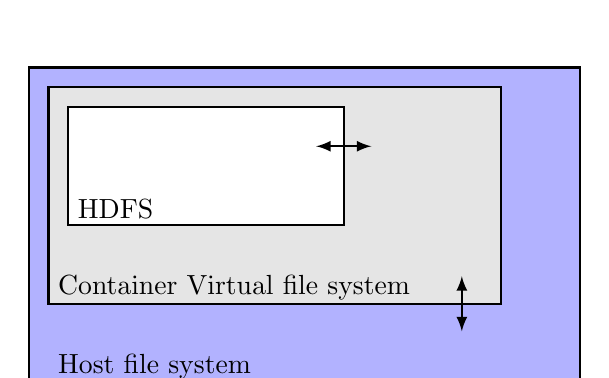
\begin{tikzpicture}[>=latex]
				\fill[draw=black, thick, fill=blue!30!white] (0,0) rectangle (7,4);\node[anchor=west] at (0.25,0.2) {Host file system};
				\fill[draw=black, thick, fill=lightgray] (0.25,1) rectangle (6,3.75);\node[anchor=west] at (0.25,1.2) {Container Virtual file system};
				\fill[draw=black, thick, fill=white] (.5,2) rectangle (4,3.5);\node[anchor=west] at (0.5,2.2) {HDFS};
				\draw[<->,thick] (5.5,.65) -- (5.5,1.35);\draw[<->,thick] (3.65,3) -- (4.35,3);
			\end{tikzpicture}
			\caption{File system organization}
			\label{tikz:filesys}
		\end{figure}

		For the installation of Docker, the Cloudera Docker image and the execution of jobs using jar file it have been used the instructions of the course. The project is written using Java version \texttt{11.0.4}. For the code compilation we used IntelliJ version \texttt{2019.2.4} compiling using compatibility mode with version \texttt{1.7}.

		Machine specifications:
		\begin{itemize}
			\item Machine 1:\begin{itemize}
			\item Operating System: \texttt{Ubuntu 16.04 LTS}, Kernel version \texttt{4.4.0-169-generic}, 64bit
			\item Processor:\texttt{Intel Core\texttrademark\ i7-4510U CPU @ 2.00GHz x4}
			\item Memory: \texttt{8 GB}
		\end{itemize} 
			\item Machine 2: \begin{itemize}
				\item Operating System: \texttt{Linux Manjaro}, Kernel version \texttt{5.3.12}, 64bit
				\item Processor:  \texttt{Intel Core\texttrademark\ i7-5500U CPU @ 3.70GHz x2}
				\item Memory: \texttt{12 GB}
			\end{itemize}
		\end{itemize}
		

		

	\subsection{Map Reduce Framework}
		MapReduce is a programming paradigm which works on parallel platforms in order to process large amounts of data in the best possible way. The client has to implement a map function, which is supposed to take raw data as input and process them into intermediate \textit{key-value} pairs, and the reduce function, which aim is to regroup key-value pairs relying on the key and generate key-value output pairs. The MapReduce model is explained more in detail in the next section.
		
		\bigskip

		\noindent
		This Programming Model consists of two main actions:
		\begin{itemize}
			\item \textbf{Map}: application of a function to every object in a list. Each object (e.g.: document) is independent.
			\begin{itemize}
				\item Order is not important;
				\item Maps can be done in parallel since every object has no relation to each other;
				\item The function produces an intermediate result.
			\end{itemize}
			Formally the \textit{map} function can be described with the following notation: \[ map:(key_1, value_1) \to list(key_2, value_2) \]
			\item \textbf{Reduce}: grouping key-value pairs on key, and combining the intermediate results generated by Maps to produce a final result. Formally the reduce function is defined as \[ reduce:(key_2, list(value_2)) \to (key_3, value_3)  \]
		\end{itemize}

		\begin{figure}[h!]
			\centering
			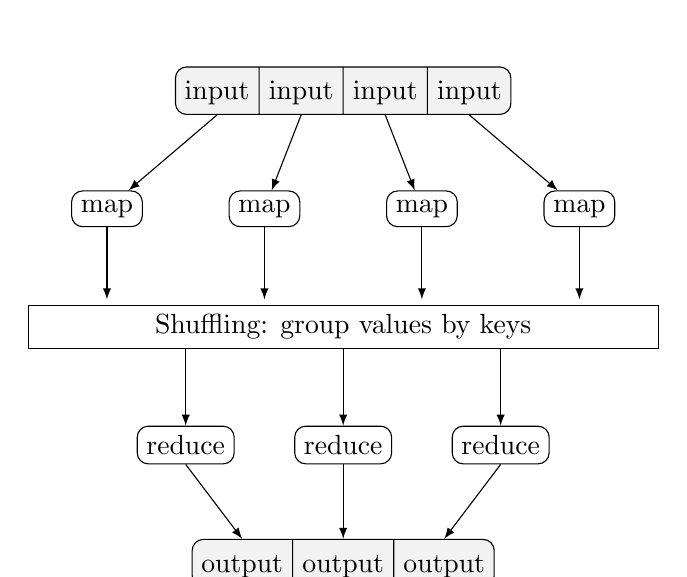
\begin{tikzpicture}[>=latex, relation/.style={rectangle split, rectangle split parts=#1, rectangle split part align=base, draw, anchor=center, align=center, text height=3mm, text centered}]
				% Nodes

				\node [relation=4, rounded corners, rectangle split horizontal, rectangle split part fill={lightgray!50}] (n0) at (0,0)
				{%
					\nodepart{one} input
					\nodepart{two} input
					\nodepart{three} input
					\nodepart{four} input};
				\node [draw, rectangle, rounded corners] (m1) at (-3,-1.5) {map};
				\node [draw, rectangle, rounded corners] (m2) at (-1,-1.5) {map};
				\node [draw, rectangle, rounded corners] (m3) at (1,-1.5) {map};
				\node [draw, rectangle, rounded corners] (m4) at (3,-1.5) {map};
				\draw node[draw, rectangle, minimum width=8cm] (inter) at ($ (n0) +(0,-3) $) {Shuffling: group values by keys};
				\node [draw, rectangle, rounded corners] (r1) at (-2,-4.5) {reduce};
				\node [draw, rectangle, rounded corners] (r2) at (0,-4.5) {reduce};
				\node [draw, rectangle, rounded corners] (r3) at (2,-4.5) {reduce};
				\node [relation=3, rounded corners, rectangle split horizontal, rectangle split part fill={lightgray!50}] (n1) at (0,-6)
				{%
					\nodepart{one} output
					\nodepart{two} output
					\nodepart{three} output};

				% Arrows

				\draw[->] (n0.one south) -- (m1);\draw[->] (n0.two south) -- (m2);
				\draw[->] (n0.three south) -- (m3);\draw[->] (n0.four south) -- (m4);
				\draw[->] (m1) -- +(0,-1.15);\draw[->] (m2) -- +(0,-1.15);
				\draw[->] (m3) -- +(0,-1.15);\draw[->] (m4) -- +(0,-1.15);
				\draw[->] ($ (inter.south) +(-2,0) $) -- (r1);\draw[->] (inter.south) -- (r2);
				\draw[->] ($ (inter.south) +(2,0) $) -- (r3);
				\draw[->] (r1.south) -- (n1.one north);
				\draw[->] (r2.south) -- (n1.two north);
				\draw[->] (r3.south) -- (n1.three north);
			\end{tikzpicture}
			\caption{MapReduce Model}
    		\label{tikz:mapred}
		\end{figure}
	
	\newpage
	\section{Project workflow and structure}\label{workflow}
	The first step of the project is to analyze an amount of manuscripts, extracting relevant information from them in order to create a ``dictionary'' of known authors. The program performs the calculation of the frequencies of english language parts most commonly used for each text and counts the most common words for each author, excluding the ones counted in the previous step.
	
	Starting from these data, the following phases consist of taking unknown manuscripts as input and establishing the authorship by the comparing them with the ``dictionary'' previously created. 
	
	All the manuscripts are \texttt{.txt} files taken from the Project Gutenberg \parencite{Gutenberg} online library.
	The Project Workflow is the following:
	\begin{enumerate}
		\item Parsing all the files using Hadoop Map Reduce job: 
		\begin{enumerate}
			\item Mapper performs the counting of all the specified language parts in each file. These parts are ArrayList instances. The Mapper associates each language part with an integer flag set to 1. The collected data are explained more in detail in the next sections. 
			
			\item Reducer performs the counting of language parts by putting together data taken from the Mappers.
		\end{enumerate}
		\item Calculating the frequencies of language parts for each text.
		\item Calculating the most common words for each author.
		\item Obtaining an author ``identikit'' based on the texts that have been analyzed written by that specific author. The author characteristics are built merging the data resulting from the text analysis.
		\item Analyzing unknown texts and comparing them to the known author in order to have a rank of similarity between the unknown texts and the known authors.
	\end{enumerate}

	\subsection{Project structure}
		The project main folder is divided in the following directories:
		\begin{figure}[h!]
			\dirtree{%
				.1 big-data-project. 
				.2 doc\DTcomment{generated javadoc folder}. 
				.2 libs \DTcomment{Hadoop libraries}. 
				.2 report\DTcomment{project report}. 
				.2 src \DTcomment{code sources}. 
				.3 main. 
				.4 java. 
				.5 analysis. 
				.6 frequencies. 
				.7 CommonWord.java. 
				.7 FreqMapEntry.java. 
				.7 FreqMap.java. 
				.6 ranking. 
				.7 AffinityMap.java. 
				.7 Pair.java. 
				.7 Ranking.java. 
				.7 SimilarityAnalysis.java. 
				.5 hadoop. 
				.6 Authorship.java. 
				.5 Main.java. 
			}
		\end{figure}

	\subsection{Map Reduce Job}
		The project contains only a single MapReduce job, alongside with other classes to hold temporary data. The MapReduce job is implemented in a single class named \lstinline|Authorship|. In order to proceed with the implementation, the code has to import several libraries, which provide interface to the HDFS functions. These libraries are:
		\begin{figure}[H]
			\dirtree{%
				.1 libs. 
				.2 hadoop-annotations.jar. 
				.2 hadoop-common.jar. 
				.2 hadoop-core-2.6.0-mr1-cdh5.7.0.jar. 
				.2 hadoop-hdfs.jar. 
				.2 log4j-1.2.17.jar. 
			}
		\end{figure}

		Before diving into the implementation of the job, we have to assure that the current class (compiled into a \verb|jar| file), will run as an hadoop job. In order to do so, we have to add \lstinline|extends Configured implements Tool| to the class declaration.
		
		\bigskip
		\noindent
		As said in the previous sections, the client has to manually implement the map and the reduce functions, alongside with a \lstinline|run| method to configure the job itself.

	\subsubsection{Run method}
		It contains the job configuration, setting input and output paths.
		The job is configured as follows:
	
	\begin{lstlisting}[firstnumber=48, caption={Run method}, captionpos=b]
@Override
public int run(String[] args) throws Exception {
	Job job = Job.getInstance(this.getConf(), "authorship");
	job.setJarByClass(this.getClass());
	TextInputFormat.setInputPaths(job, new Path(INPUT_PATH));
	TextInputFormat.setInputPaths(job, new Path(UNKNOWNS_INPUT_PATH));
	TextOutputFormat.setOutputPath(job, new Path(OUTPUT_PATH));
	
	for (String s : Main.buildPaths(this))
		FileInputFormat.addInputPath(job, new Path(s));
	
	job.setMapperClass(Map.class);
	job.setCombinerClass(Reduce.class);
	job.setReducerClass(Reduce.class);
	job.setMapOutputKeyClass(Text.class);
	job.setMapOutputValueClass(IntWritable.class);
	job.setOutputKeyClass(Text.class);
	job.setOutputValueClass(IntWritable.class);
	
	return job.waitForCompletion(true) ? 0 : 1;
}
	\end{lstlisting}
	
		Note that several costants are used: \begin{itemize}
			\item \lstinline|INPUT_PATH| (\lstinline|/user/root/authorship/input/|) is the input path for known texts;
			\item \lstinline|OUTPUT_PATH| (\lstinline|/user/root/authorship/output/|) is the reduce output path;
			\item \lstinline|UNKNOWNS_INPUT_PATH| (\lstinline|/user/root/authorship/input/unknowns/|) is the input path for unknown texts (which are located in a subdirectory of \lstinline|INPUT_PATH|).
		\end{itemize}

		\noindent
		The calls to \lstinline|setInputPaths| and \lstinline|setOutputPath|, as the name suggests, are used to set respectively the input and output paths of the job. Then we add the single files using a call to \lstinline|addInputPath| for each input file we have. 
		
		\bigskip
		\noindent
		In the following lines, we configure the mapper and reducer input and output types and classes.
		Respectively: \begin{itemize}
			\item mapper output key is \lstinline|Text| (the hadoop-like type for \lstinline|String|);
			\item mapper output value is \lstinline|IntWritable| (standing for \lstinline|Integer|);
			\item reducer output key is \lstinline|Text|;
			\item reducer output value is \lstinline|Integer|.
		\end{itemize}

		\noindent
		The calls to \lstinline|job.setMapperClass|, \lstinline|job.setReducerClass| and \lstinline|job.setCombinerClass| just tell the interpreter which is the class responsible for describing the mapping, reducing and combining function.
		
	\subsubsection{Mapper implementation} 
		
		The mapper is implemented in an inner class, and we can summarize the content by dividing it in three sections.

		\noindent
		The first one contains the declaration of patterns during the analysis.
	
	\begin{lstlisting}[firstnumber=73, caption={Declaration of Regular Expression Patterns}, captionpos=b]
private static final Pattern WORD_BOUNDARY = Pattern.compile("\\s*\\b\\s *");
private static final Pattern END_PERIOD = Pattern.compile("[a-z][.!?]");
private static final Pattern MARKS_COMMAS = Pattern.compile("[,!?]");
private static final IntWritable ONE = new IntWritable(1);
	\end{lstlisting}
	
		\noindent
		These pattern are used in the text analysis. Briefly: \begin{itemize}
			\item \lstinline|WORD_BOUNDARY|: splits on word separators characters;
			\item \lstinline|END_PERIOD|: splits text on end-period characters;
			\item \lstinline|MARKS_COMMAS|: splits on commas and exclamation/question marks;
		\end{itemize}

	\noindent
	The last constant is an \lstinline|IntWritable| value set to 1, and is used when a matching expression is detected.

	\noindent
	The second section contains the text analysis itself, which is based on: \begin{itemize}
		\item articles, prepositions, conjunctions, verbs and pronouns frequency;
		\item average period length;
		\item punctuation mark frequency.
	\end{itemize}
	Besides this, we save additional information, such as the total number of words in the input and the total number of periods, so we can get the frequency over the total dimension of the input.

	In this section the previous pattern matchers are used to reach these words and write the corresponding \lstinline|ONE| in the job contest. 
	
	We report an example for articles count: \begin{lstlisting}[firstnumber=85, caption={Articles counting in Map method}, captionpos=b]
for (String word : WORD_BOUNDARY.split(lineText.toString())) {
	String refWord = word.toLowerCase();
	if (!word.isEmpty()) {
		if (Authorship.ARTICLES.contains(refWord)) {
			text.set(filePathString + "*article");
			context.write(text, ONE);
		}
	}

	...

}
	\end{lstlisting}
	
	In short terms, for each article found in the input text, the mapper writes a string formatted as follows:\begin{center}
		\texttt{author-title.txt*article<tab><value>} 
	\end{center}

	This procedure applies in the same way to preposition, conjunctions and other language parts.
	
	\bigskip
	\noindent
	For periods and punctuation we used a different method.
	\begin{lstlisting}[firstnumber=109, caption={Periods counting in Map method}, captionpos=b]
Matcher matcher = END_PERIOD.matcher(refLineText);
while (matcher.find()) {
	text.set(filePathString + "*periods");
	context.write(text, ONE);
}
	...
	\end{lstlisting}
	
	A \lstinline|Matcher| instance tries to match the pattern to an input line. As soon as the matcher finds occurences of the pattern in the text passed as parameter, the mapper writes a line similar to the previous one (i.e. formatted in the same way) to the context. The procedure repeats for punctuation marks, commas and periods delimitators. \\
	
	At last the mapper performs the count of the words which have not been counted in the previous matchings. The code running this task is the following:
	\begin{lstlisting}[firstnumber=119, caption={Common words counting in the Map method.}, captionpos=b]
Matcher commonWordsMatcher = COMMONS.matcher(lineText.toString());
while (commonWordsMatcher.find()) {
	String w = commonWordsMatcher.group().toLowerCase();
	if (!Authorship.ARTICLES.contains(w) && ... &&
		!Authorship.VERBS.contains(w)) {
			text.set(filePathString + "*commons:" + w);
			context.write(text, ONE);
	}
}
		
	\end{lstlisting}
	
	The string used to format the common words is a bit different: \begin{center}
		\texttt{author-title.txt*common:<word><tab><value>}
	\end{center}
	
	\subsubsection{Reducer implementation}
		The reducer implementation is pretty much the same as in the \lstinline|Wordcount| example. Since it's just a few lines we report the full code:
	\begin{lstlisting}[firstnumber=152, caption={Reduce method}, captionpos=b]
@Override
protected void reduce(Text key, Iterable<IntWritable> values, Context context) throws IOException, InterruptedException {
	int sum = 0;
	for (IntWritable count : values) {
		sum += count.get();
	}
	context.write(key, new IntWritable(sum));
}
	\end{lstlisting}
	
		Since the context has now a lot of lines associated with same value (the \lstinline|IntWritable| instance for ``ones''), the combiner and the reducer are responsible for grouping lines with the same key and count these lines, writing the total into the context.
		
		For the common words, the reducer counts all the occurrences of the same word for an author in a text.
	
	\subsection{Frequency Calculations}
		Once the hadoop job has terminated, the control switches to a simple Java program. This section of the program generates an instance of the class \lstinline|FreqMap| (implemented as a singleton) which parses the reducer output file and builds a set of \lstinline|FreqMapEntries|.
		
		\noindent
		A \lstinline|FreqMap| instance is a set of \lstinline|FreqMapEntry|, which are text-specific entries. More in detail an instance of \lstinline|FreqMapEntry| consists of: \begin{itemize}
			\item A \lstinline|String| author name;
			\item A \lstinline|String| text title;
			\item A map \lstinline|String| $\to$ \lstinline|Float|, containing field names (text features extracted from the MapReduce framework) and their respective values;
			\item  A list of \lstinline|String| instances, which contains the most common words for the text specified in the title.
		\end{itemize}

		\noindent
		More in detail, the map from strings to float contains the following fields: \begin{itemize}
			\item Frequency of articles;
			\item Frequency of prepositions;
			\item Frequency of conjunctions;
			\item Frequency of verbs;
			\item Frequency of pronouns;
			\item Number of words in the input;
			\item Number of periods in the input;
			\item Frequency of punctuation marks;
			\item Average period length.
		\end{itemize}

		\noindent
		Note that the frequency of articles, prepositions, conjunctions, verbs, pronouns and punctuation symbols is determined over the total number of words.
		
		\noindent
		After this phase, we will have a frequency map for every text of every author, for example:

	\begin{figure}[h!]
		\centering
		\begin{BVerbatim}[fontsize=\small]
ENTRY: dickens global
	periods             5079.822
	avg_period_length     23.619436
	articles               0.067365
	conjunctions           0.058276057
	pronouns               0.116758764
	verbs                  0.05449821
	commas                 0.084043525
	nwords            110616.18
	prepositions           0.11444762

Common Words:
	mr      0.0030926832
	old     0.001698533
	man     0.0016119949
	time    0.0014565586
	never   0.0011964154
	good    0.0011850407
	before  0.0011834776
	know    0.001170031
	than    0.001152259
	great   0.0011296555
	\end{BVerbatim}
\end{figure}

		\noindent
		What we need now is a map of frequencies relative to a single author, in order to generate a ``stylistic identikit''  of an author, so then we can compare any unknown text to that author.

		\noindent
		In order to do so we pick all the information we got about every known text of every author and we merge this maps into a single one, which is relative to an author. That is, if we have multiple texts of the same author, we generate a new \lstinline|FreqMapEntry|, were the author remains the same, but we set as title a \lstinline|String| set to the value \lstinline|"global"|, in order to identify that map as the author identikit we were talking some lines above.

		\bigskip
		\noindent
		The global entries are generated with the method named \lstinline|globalAuthorFrequency()|, which performs, in order, the following tasks: \begin{enumerate}
		\item Merges all the common words from the same author into a one, huge list, orders these words by their frequency and keeps the first ten words;
		\item Calculates, for each field of the map, the average values for the different language parts, and fills the global entry with the average values;
		\item Creates a new \lstinline|FreqMapEntry| with the results of points 1 and 2.
		\end{enumerate}

		\bigskip
		\noindent
		At the end we will have in the beginning \lstinline|FreqMap| instance an entry for each text of each author and a global entry for every author.
	
	\subsection{Similarity Analysis}
		The last phase of the working project is the design of the mechanism which allows to attribute an hypothetical author to an unknown text.
		
		\noindent
		The task is done through the following steps: 
		\begin{enumerate}
			\item Generating a partial comparison between every couple of unknown text-known author;
			\item Sorting this comparisons in order to get the most similar couples as the most correlated author to each unknown text.
		\end{enumerate}

		\noindent
		This steps are implemented in \lstinline|AffinityMap| and \lstinline|SimilarityAnalysis| classes.
		
		\noindent
		An \lstinline|AffinityMap| instance represents a comparison of authors, the first is known and the second is not. The compared fields are represented as a map \lstinline|String| $\to$ \lstinline|Double|, as in previous classes. The \lstinline|AffinityMap| instance implements the \lstinline|Comparable| interface, in order to be able to compare two instances and determine a sort of ``hierarchy''.
		
		\noindent
		The comparison method is the following:
		\begin{lstlisting}[firstnumber=51,caption={AffinityMap comparison method}, captionpos=b, label={lst:comparemethod}]
@Override
public int compareTo(Object o) {
	AffinityMap rec = (AffinityMap) o;
	HashMap<Integer, Integer> count = new HashMap<>();(*@\label{54}@*)
	count.put(-1, 0);
	count.put(0, 0);
	count.put(1, 0);(*@\label{57}@*)
	
	// count for compare values
	for (String s : this.map.keySet()) {(*@\label{60}@*)
		if (this.map.get(s) < rec.map.get(s)) {
			count.put(-1, count.get(-1) + 1);
		} else if (rec.map.get(s) < this.map.get(s)) {
			count.put(1, count.get(1) + 1);
		} else {
			count.put(0, count.get(0) + 1);
		}
	}(*@\label{68}@*)
	
	// max on compare counts
	Map.Entry<Integer, Integer> max = null;
	int intmax = 0;(*@\label{72}@*)
	for (Map.Entry<Integer, Integer> entry : count.entrySet()) {
		if (entry.getValue() > intmax) {
			intmax = entry.getValue();
			max = entry;
		}
	}(*@\label{78}@*)
	assert max != null;
	return max.getKey();

}
	 \end{lstlisting}
	 
	 \noindent
	We break the above written code down to its basics. Before we dive into it, we have to recall the functioning of the standard \lstinline|compareTo(Object o)| method, inherited from the \lstinline|Comparable| interface. This method returns \begin{itemize}
		\item $0$ if the objects are equal;
	 	\item $-1$ if \lstinline|this| object is lower then the parameter object;
	 	\item $1$ if \lstinline|this| object is greater then the parameter object;
	\end{itemize}
 
	\noindent
	 Now we can explain the code more in detail: 
	\begin{itemize}
 		\item Lines \ref{54} :: \ref{57} initialize to 0 three counters, one for each return type of the \lstinline|compare| method;
 		\item Lines \ref{60} :: \ref{68} compare each field of the two maps (which have the same key) and increment the corresponding counter;
 		\item Lines \ref{72} :: \ref{78} check which of the three counter has the maximum value; if $-1$ is the maximum, the current object is lower that the parameter item, if $1$ is the maximum the parameter item is lower than the current object, otherwise the two items are considered to be equal.
 	\end{itemize}
 	The comparison is run from the method \lstinline|SimilarityAnalysis.exec()|, which is responsible for generating the correlations between unknown text and known authors and reporting to file the final rank. We start the description of the class from specifying how affinities are calculated, and report the \lstinline|exec()| method code.
 	
 	\begin{lstlisting}[firstnumber=38]
private void exec() {
	// remove non globals values and sort entries
	ArrayList<FreqMapEntry> unknowns = new ArrayList<>();
	ArrayList<FreqMapEntry> knowns = new ArrayList<>();
	
	for (FreqMapEntry entry : this.freqMap.getEntries()) {(*@\label{43}@*)
		if (entry.isUnknown() && entry.isGlobal()) {
			unknowns.add(entry);
		} else if (!entry.isUnknown() && entry.isGlobal()) {
			knowns.add(entry);
		}
	}
	
	// calc deltas for each FreqMapEntry combination
	for (FreqMapEntry kn : knowns) {
		for (FreqMapEntry unk : unknowns) {
			this.deltas.add(computedDelta(kn, unk));
		}
	}(*@\label{56}@*)
	
	Collections.sort(this.deltas, new Comparator<AffinityMap>() {(*@\label{58b}@*)
		// comparison method between two affinity maps, used to sort the analysis
		@Override
		public int compare(AffinityMap affinityMap, AffinityMap t1) {
			return affinityMap.compareTo(t1);
		}
	});(*@\label{64b}@*)
}
 	\end{lstlisting}
 	
 	\bigskip
 	\noindent
	As specified just few lines above, an \lstinline|AffinityMap| instance contains a map from String to doubles. The data in this map are saved as the field-to-field difference of the maps of the authors we are analyzing. More in detail, if we have two authors $A$ and $B$ (i.e. two \lstinline|FreqMapEntry| instances), the map will contain the following values (lines \ref{43} to \ref{56}):
	\begin{align*}
		\begin{cases}
			\text{articles} &= |A.\text{articles} - B.\text{articles}| \\
			\text{conjunctions} &= |A. \text{conjunctions}- B.\text{conjunctions}| \\
			\dots& \\
			\text{avg-period-length}&= |A.\text{avg-period-length} - B.\text{avg-period-length}|
		\end{cases}
	\end{align*}
	
	\noindent
	Lines \ref{58b} to \ref{64b} sort the collection of \lstinline|AffinityMap| instances using the \lstinline|compare| method described in listing \ref{lst:comparemethod}.
	
	\noindent
	The ranking is written to a new file in the HDFS (in directory \lstinline|OUTPUT_PATH|); the first position are the most similar, the last position are the smallest affinity pairs.
	
	\newpage
	\section{Running on a sample}\label{sample}
	\subsection{Extracted data}
	During the development process, we tested the program on a bunch of samples (240 files, more or less 94 MB) from 3 different authors: 
	\begin{itemize}
		\item Jacob Abbott -- 47 texts (plus three unknown texts marked as Unknown1, Unknown2 and Unknown3);
		\item Charles Dickens -- 101 texts (plus two unknown texts marked as Unknown4 and Unknown5);
		\item Robert Louis Stevenson -- 80 texts (plus one unknown text marked as Unknown6).
	\end{itemize}

		\noindent
		These texts are taken from the Project Gutenberg online library. Each text is formatted as an utf8 plain-text txt file.

		\bigskip

		\noindent
		We used most common words used by authors as the most relevant parameter to check authorship. In this case all unknown texts are correctly recognized. If the most common words are the same in the unknown text and in more than one author ``dictionary'' of texts, this check is irrelevant. So we decided to consider period length as the second parameter of recognition. At last if the period length check is irrelevant too, we count each article, preposition, conjunction, pronoun, verb and punctuation mark frequency.

		\noindent
		Running the program on the known texts, we got the following information:
		\begin{table}[h!]
			\small
			\begin{tabular}{lcccccc}
				\toprule
				Author   & Articles    & Conjunctions & Pronouns & Verbs & Prepositions &   Commas  \\
				\midrule
				J.Abbott      & 0.082  & 0.065 & 0.117 & 0.067 & 0.134 & 0.076  \\
				C.Dickens     & 0.067  & 0.058 & 0.116 & 0.054 & 0.114 & 0.084  \\
				R.L.Stevenson & 0.079  & 0.059 & 0.110 & 0.053 & 0.119 & 0.074  \\
				\bottomrule
			\end{tabular}
			\caption{Frequencies in known authors' texts}
			\label{tab:known-freq}
		\end{table}
		\bigskip

		\noindent
		Running the program on unknown texts, we obtained the following data:
		\begin{table}[h!]
			\small
			\begin{tabular}{cccccccc}
				\toprule
				Number & Articles & Conjunctions & Pronouns & Verbs & Prepositions & Commas \\
				\midrule
				Unknown1 & 0.076 & 0.068 & 0.126 & 0.082 & 0.111 & 0.095 \\
				Unknown2 & 0.092 & 0.062 & 0.105 & 0.057 & 0.149 & 0.071 \\
				Unknown3 & 0.100 & 0.056 & 0.100 & 0.059 & 0.143 & 0.078 \\
				Unknown4 & 0.058 & 0.063 & 0.141 & 0.058 & 0.114 & 0.107 \\
				Unknown5 & 0.065 & 0.061 & 0.124 & 0.058 & 0.113 & 0.087 \\
				Unknown6 & 0.097 & 0.076 & 0.132 & 0.075 & 0.109 & 0.075 \\
				\bottomrule
			\end{tabular}
			\caption{Frequencies in unknown authors' texts}
			\label{tab:unknown-freq}
		\end{table}

	\newpage
	\subsection{Results and analysis}

	\subsubsection{Global Frequencies for all authors}

	\begin{figure}[h!]
		\centering
		\begin{tikzpicture}
			\begin{axis}
			[
			legend entries={Abbott, Dickens, Stevenson},
			legend style={
				at={(1.5,-0.2)},
				anchor=north,
				legend columns=1,
				cells={anchor=west},
				font=\footnotesize,
				rounded corners=2pt,
			},
			grid=major,
			height=7cm,
			grid style={densely dotted},
			ymin=1,
			xtick=data,
			ytick={1, 3, ..., 16},
			legend pos=outer north east,
			yticklabel={\pgfmathprintnumber{\tick}\,\%},
			x tick label style={rotate=90},
			xticklabels={articles,conjunctions,pronouns,verbs,prepositions,punctuation},
			ylabel=Frequencies]
			\addplot table [x=freq, y=abbott, col sep=comma] {csv-files/frequencies.csv};
			\addplot table [x=freq, y=dickens, col sep=comma] {csv-files/frequencies.csv};
			\addplot[mark=*, brown] table [x=freq, y=stevenson, col sep=comma] {csv-files/frequencies.csv};
			\end{axis}
		\end{tikzpicture}
		\caption{Language parts frequencies of all authors in all texts}
		\label{tikz:frequencies}
	\end{figure}

	\subsubsection{Frequencies between known and uknown authors}

	\begin{figure}[h!]
		\centering
		\begin{tikzpicture}
			\begin{polaraxis}
			[
			legend entries={Abbott, Unknown1, Unknown2, Unknown3},
			legend style={
				at={(1.5,-0.2)},
				anchor=north,
				legend columns=1,
				cells={anchor=west},
				font=\footnotesize,
				rounded corners=2pt,
			},
			grid=major,
			height=9cm,
			grid style={thick,densely dotted},
			yshift=0.5cm,
			xshift=100,
			xtick=data,
			ytick={0, 3, ..., 19},
			legend pos=outer north east,
			yticklabel={\footnotesize\pgfmathprintnumber{\tick}},
			xticklabels={articles,conjunctions,pronouns,verbs,prepositions,punctuation}]
			\addplot table [data cs=polarrad, x=freq, y=abbott, col sep=comma] {csv-files/abbott-unknown.csv};
			\addplot table [data cs=polarrad, x=freq, y=unknown1, col sep=comma] {csv-files/abbott-unknown.csv};
			\addplot table [data cs=polarrad, x=freq, y=unknown2, col sep=comma] {csv-files/abbott-unknown.csv};
			\addplot table [data cs=polarrad, x=freq, y=unknown3, col sep=comma] {csv-files/abbott-unknown.csv};
			\end{polaraxis}
		\end{tikzpicture}
		\caption{Frequencies between Abbott and 3 unknowns.\\
		We can observe that there is quite a similarity between Abbott frequencies and the unknown authors' texts. The only difference is the use in prepositions in the Unknown3 text, but it is still included in deltas intervals.}
		\label{tikz:abbott-unk}
	\end{figure}
	  

	\begin{figure}[h!]
		\centering
		\begin{tikzpicture}
			\begin{polaraxis}
			[
			legend entries={Dickens, Unknown4, Unknown5},
			legend style={
				at={(1.5,-0.2)},
				anchor=north,
				legend columns=1,
				cells={anchor=west},
				font=\footnotesize,
				rounded corners=2pt,
			},
			grid=major,
			height=9cm,
			grid style={thick,densely dotted},
			xtick=data,
			ytick={0, 3, ..., 19},
			legend pos=outer north east,
			yticklabel={\footnotesize\pgfmathprintnumber{\tick}},
			xticklabels={articles,conjunctions,pronouns,verbs,prepositions,punctuation}]
			\addplot table [data cs=polarrad, x=freq, y=dickens, col sep=comma] {csv-files/dickens-unknown.csv};
			\addplot table [data cs=polarrad, x=freq, y=unknown4, col sep=comma] {csv-files/dickens-unknown.csv};
			\addplot table [data cs=polarrad, x=freq, y=unknown5, col sep=comma] {csv-files/dickens-unknown.csv};
			\end{polaraxis}
		\end{tikzpicture}
		\caption{Frequencies between Dickens and 2 unknowns\\
		We can observe that there is quite a similarity between Dickens frequencies and the unknown authors' texts.}
		\label{tikz:dickens-unk}
	\end{figure}

	\begin{figure}[h!]
		\centering
		\begin{tikzpicture}
			\begin{polaraxis}
			[
			legend entries={Stevenson, Unknown6},
			legend style={
				at={(1.5,-0.2)},
				anchor=north,
				legend columns=1,
				cells={anchor=west},
				font=\footnotesize,
				rounded corners=2pt,
			},
			grid=major,
			height=9cm,
			grid style={thick,densely dotted},
			xtick=data,
			ytick={0, 3, ..., 19},
			legend pos=outer north east,
			yticklabel={\footnotesize\pgfmathprintnumber{\tick}},
			xticklabels={articles,conjunctions,pronouns,verbs,prepositions,punctuation}]
			\addplot table [data cs=polarrad, x=freq, y=stevenson, col sep=comma] {csv-files/stevenson-unknown.csv};
			\addplot table [data cs=polarrad, x=freq, y=unknown6, col sep=comma] {csv-files/stevenson-unknown.csv};
			\end{polaraxis}
		\end{tikzpicture}
		\caption{Frequencies between Stevenson and 1 unknown\\
		We can observe that there is quite a similarity between Stevenson frequencies and the unknown author's text.}
		\label{tikz:stevenson-unk}
	\end{figure}
	
	\subsubsection{Deltas differences between known and unknown authors}
	\begin{figure}[h!]
		\centering
		\begin{tikzpicture}
			\begin{axis}
			[
			legend entries={Abbott, Unknown1, Unknown2, Unknown3},
			legend style={
				at={(1.5,-0.2)},
				anchor=north,
				legend columns=1,
				cells={anchor=west},
				font=\footnotesize,
				rounded corners=2pt,
			},
			grid=major,
			height=8cm,
			grid style={densely dotted},
			ymin=-1,
			xtick=data,
			ytick={0, 3, ..., 16},
			legend pos=outer north east,
			yticklabel={\pgfmathprintnumber{\tick}\,\%},
			x tick label style={rotate=90},
			xticklabels={articles,conjunctions,punctuation,prepositions},
			ylabel=Deltas]
			
			\addplot[ultra thick, black] table [mark=none, x=freq, y=abbott, col sep=comma] {csv-files/deltas-abbott.csv};
			\addplot[mark=none,blue] table [ x=freq, y=unknown1, col sep=comma] {csv-files/deltas-abbott.csv};
			\addplot[mark=none,red] table [ x=freq, y=unknown2, col sep=comma] {csv-files/deltas-abbott.csv};
			\addplot[mark=none,green] table [ x=freq, y=unknown3, col sep=comma] {csv-files/deltas-abbott.csv};
			\addplot[error bars/.cd, y explicit, y dir=minus, error bar style={dashed,red, line width=1pt},
				error mark options={mark=none} ] table [x=freq, y=abbott, y error minus expr=\thisrow{abbott}-\thisrow{unknown1},
				col sep=comma ] {csv-files/deltas-abbott.csv};
			\addplot[error bars/.cd, y explicit, y dir=minus, error bar style={dashed,red, line width=1pt},
				error mark options={mark=none} ] table [x=freq, y=abbott, y error minus expr=\thisrow{abbott}-\thisrow{unknown2},
				col sep=comma ] {csv-files/deltas-abbott.csv};
			\addplot[error bars/.cd, y explicit, y dir=minus, error bar style={dashed,red, line width=1pt},
				error mark options={mark=none} ] table [x=freq, y=abbott, y error minus expr=\thisrow{abbott}-\thisrow{unknown3},
				col sep=comma ] {csv-files/deltas-abbott.csv};
			\end{axis}
		\end{tikzpicture}
		\caption{Abbott differences between Abbott known texts and other Abbott texts marked as unknown}
		\label{tikz:abbott-deltas}
	\end{figure}

	\begin{figure}[h!]
		\centering
		\begin{tikzpicture}
			\begin{axis}
			[
			legend entries={Dickens, Unknown4, Unknown5},
			legend style={
				at={(1.5,-0.2)},
				anchor=north,
				legend columns=1,
				cells={anchor=west},
				font=\footnotesize,
				rounded corners=2pt,
			},
			grid=major,
			height=8cm,
			grid style={densely dotted},
			ymin=-1,
			xtick=data,
			ytick={0, 3, ..., 16},
			legend pos=outer north east,
			yticklabel={\pgfmathprintnumber{\tick}\,\%},
			x tick label style={rotate=90},
			xticklabels={articles,conjunctions,punctuation,prepositions},
			ylabel=Deltas]
			
			\addplot[ultra thick, black] table [mark=none, x=freq, y=dickens, col sep=comma] {csv-files/deltas-dickens.csv};
			\addplot[thick,mark=none,blue] table [ x=freq, y=unknown4, col sep=comma] {csv-files/deltas-dickens.csv};
			\addplot[thick,mark=none,green] table [ x=freq, y=unknown5, col sep=comma] {csv-files/deltas-dickens.csv};
			\addplot[error bars/.cd, y explicit, y dir=minus, error bar style={dashed,red, line width=1pt},
			 error mark options={mark=none} ] table [x=freq, y=dickens, y error minus expr=\thisrow{dickens}-\thisrow{unknown5},
				col sep=comma ] {csv-files/deltas-dickens.csv};
			\addplot[error bars/.cd, y explicit, y dir=minus, error bar style={dashed,red, line width=1pt},
				error mark options={mark=none}] table [x=freq, y=dickens, y error minus expr=\thisrow{dickens}-\thisrow{unknown4},
				col sep=comma] {csv-files/deltas-dickens.csv};
			\end{axis}
		\end{tikzpicture}
		\caption{Deltas differences between Dickens known texts and other Dickens texts marked as unknown}
		\label{tikz:dickens-deltas}
	\end{figure}

	\clearpage
	
	\section{Designing choices}\label{designing choices}
	During the development process we encountered several issues and in order to solve them, we implemented some restrictive design choices.
	
	\begin{itemize}
		\item \textbf{Environment:} we spent quite some time to make hadoop work on linux. In fact, there seem to be some problems in running hadoop on Arch-based distributions (expecially the webserver part). 
		
		Besides that, we noticed that some particular hardware configuration make hadoop crash or not work properly, we fixed by manually changing the amount of memory reserved to hadoop, in its configuration files. In particular in the machine 1, with 8 GB of Memory, we had to configure the \texttt{/etc/hadoop/conf/yarn-site.xml} file adding the following options: 
		\begin{itemize}
			\item Maximum percentage of disk utilization with value 100.0;
			\item Minimum percentage of disk utilization with value 0.0;
			\item Minimum limit of memory to allocate to each container request at the Resource Manager with value 1024;
			\item Maximum limit of memory to allocate to each container request at the Resource Manager with value 4096;
			\item Physical memory, in MB, to be made available to running containers with value 4096;
			\item Number of CPU cores that can be allocated for containers with value 4;
			\item The minimum allocation for every container request at the RM, in terms of virtual CPU cores with value 1. Requests lower than this won't take effect, and the specified value will get allocated the minimum;
			\item The maximum allocation for every container request at the RM, in terms of virtual CPU cores with value 5. Requests higher than this won't take effect, and will get capped to this value.
		\end{itemize}
		
		\item \textbf{Virtualized filesystem access:} the access to the effective filesystem needed in order to manipulate files is quite tricky, in fact the filesystem reserved to the process is retrievable only by a specific call to the job configuration and the documentation is quite difficult to understand.
		
		\item \textbf{Input file naming format:} due to difficulties in the parsing process, we decide to format the input file names \texttt{author-title.txt}, and the unknown files as \texttt{unknown-unknown.txt}.
	\end{itemize}

	\subsection{Predefined paths and program running}
	Since we embedded input and output paths directly in the code, we have to give the directory structure we used throughout the development process. 
	\begin{figure}[h!]
		\dirtree{%
			.1 user.
			.2 root.
			.3 authorship.
			.4 input\DTcomment{input file folder}.
			.5 unknowns\DTcomment{unknowns input file folder}.
			.4 output\DTcomment{output file folder}.
		}
	\caption{Hadoop directory tree.}
	\end{figure}

	With this directory structure, a possible user has just to place the files in the right directory (\lstinline|unknowns| if the text is unknown or in \lstinline|input| if the author is known) simply run the program.
	
	In order to run the program we wrote down a quick script, named \lstinline|exec.sh| which deletes the output directory, runs the jar file and cats the output properly ``grepped''.

	\subsection{Performance considerations} % 7m24s
	The running time of the whole job is around 7 minutes. The number of mappers is always equal to the number of input texts and there is always only one reducer.
	

	\newpage
	\printbibheading
	\printbibliography[nottype=book,heading=subbibliography,title={Online Sources}]





\end{document}